\subsection{Experimental overview of Bottomonia results at RHIC and LHC}

%\subsubsection{Proton-proton collisions as a reference for R$_{AA}$ at the LHC}

\subsubsection{$\Upsilon$(nS) R$_{AA}$ at the LHC}

\paragraph{Measurement by CMS, ATLAS and ALICE}

The bottomonia states ($\Upsilon$(nS)) are measured at the LHC with very good statistical
precision~\cite{Chatrchyan:2012lxa,Abelev:2014nua,Chatrchyan:2011pe,Khachatryan:2016xxp}.
The CMS measurements at $\sNN =$2.76 TeV~\cite{Chatrchyan:2012lxa,Chatrchyan:2011pe} reveal
a clear proof of sequential suppression :  $\Upsilon$(2S) and $\Upsilon$(3S) are 
more suppressed relative to the ground state $\Upsilon$(1S).   The individual $\Upsilon$ states are also found to be suppressed in
the PbPb collisions relative to the production in the pp collisions. The $\Upsilon$ nuclear
modification factor, $R_{AA}$, shows a strong dependence on collision centrality but has
weak dependence on $\Upsilon$ meson $\pT$ and rapidity~\cite{Khachatryan:2016xxp}.
The forward rapidity ($2.5 \leq y^{\Upsilon} \leq 4.0$) measurement of the $\Upsilon$ suppression at 
ALICE~\cite{Abelev:2014nua} is found to be consistent with the midrapidity ($|y^{\Upsilon}|\,\leq 2.4$)
measurement of the $\Upsilon$ suppression at the CMS. 
The CMS and ALICE collaborations have carried out the $R_{AA}$ measurement of $\Upsilon$
at $\sNN =$ 5.02 TeV with the Run II LHC PbPb
collisions~\cite{Sirunyan:2018nsz,Sirunyan:2017lzi,ALICE:Y5TeV}.
The CMS experiment measured slightly more amount of $\Upsilon$ suppression at
$\sNN =$ 5.02 TeV~\cite{Sirunyan:2018nsz,Sirunyan:2017lzi} than the suppression at
$\sNN =$ 2.76 TeV~\cite{Khachatryan:2016xxp} while the ALICE experiment observed less
suppression at $\sNN =$ 5.02 TeV than that at $\sNN =$ 2.76 TeV 
in the most central PbPb collisions~\cite{Abelev:2014nua,ALICE:Y5TeV}.

\subsubsection{$\Upsilon$(nS) azimuthal anisotropy at the LHC}

\begin{figure}
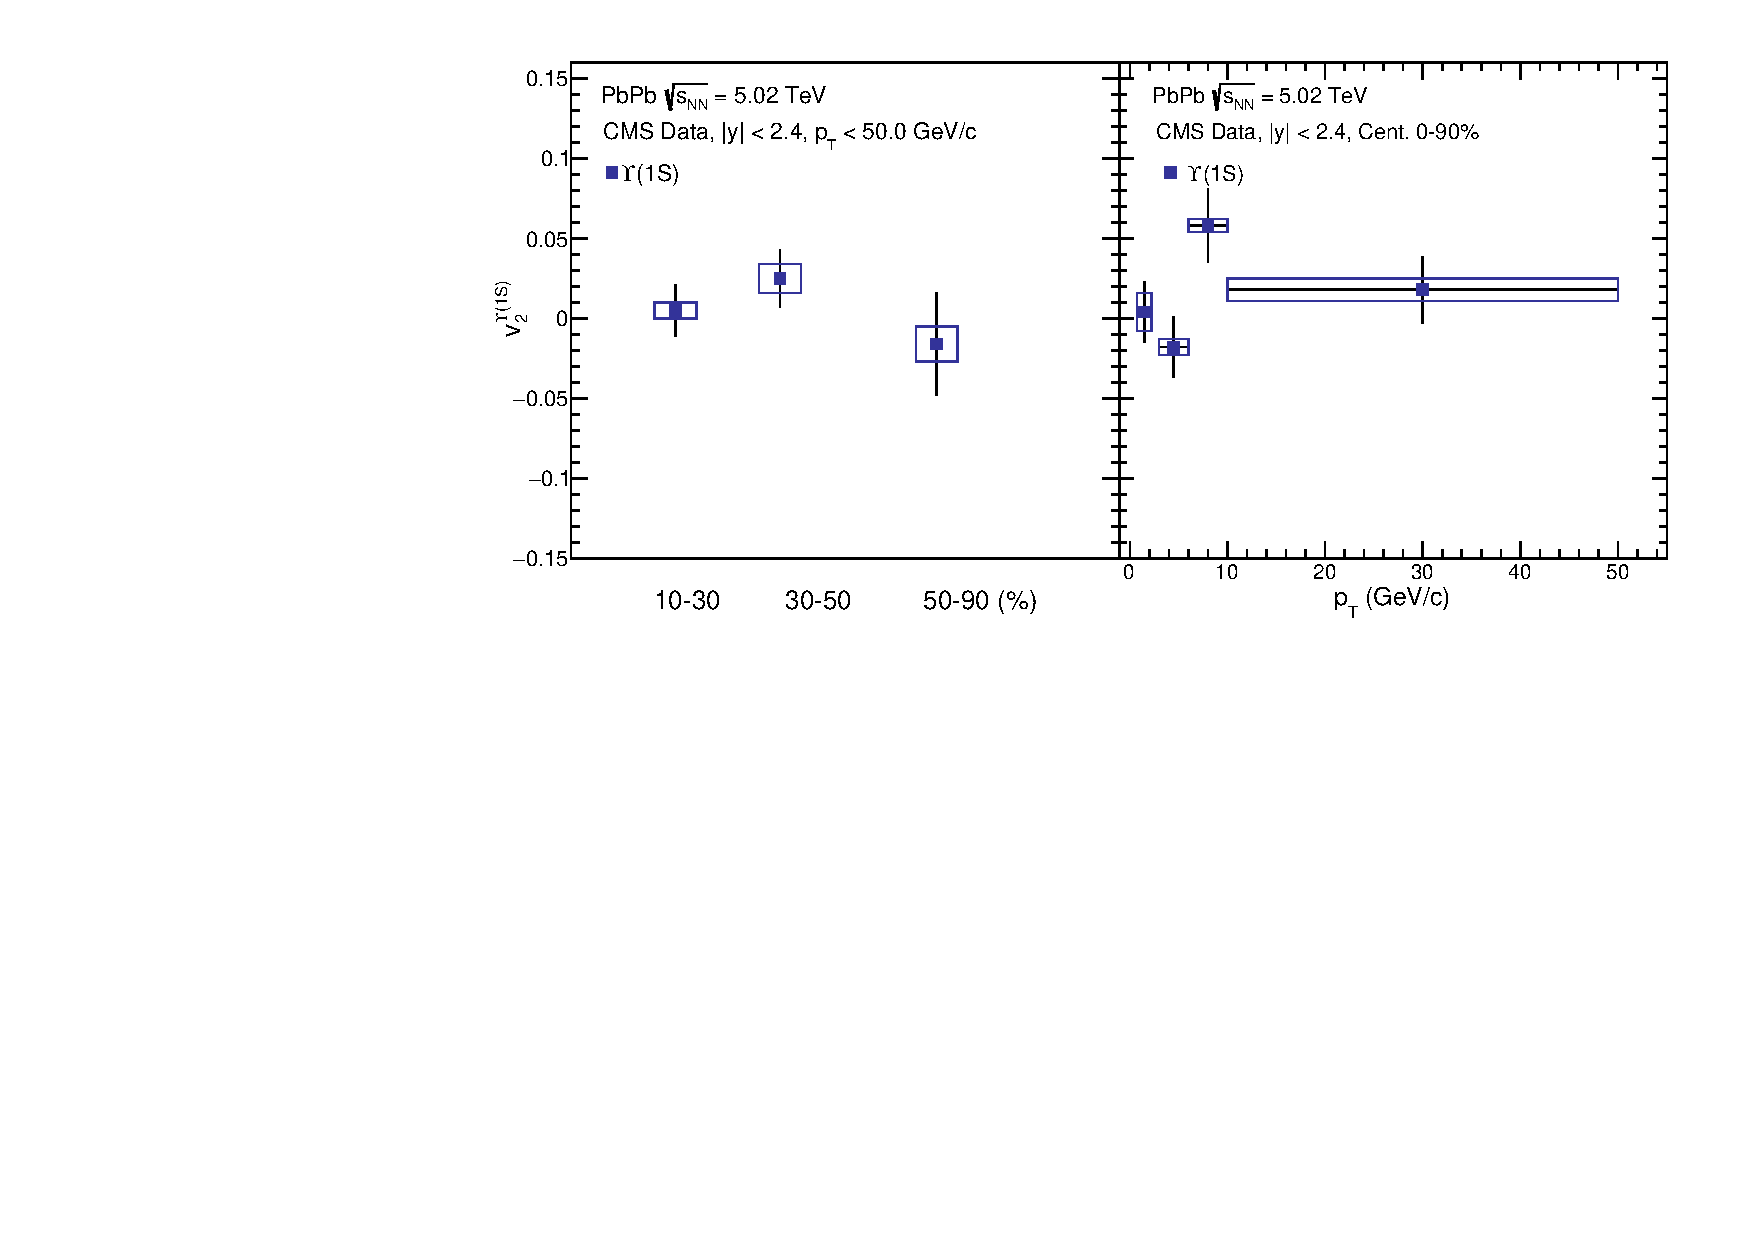
\includegraphics[width=0.99\textwidth]{Figures/ExpOverview/Fig_CMS_Y1S_5TeV_V2.pdf}
%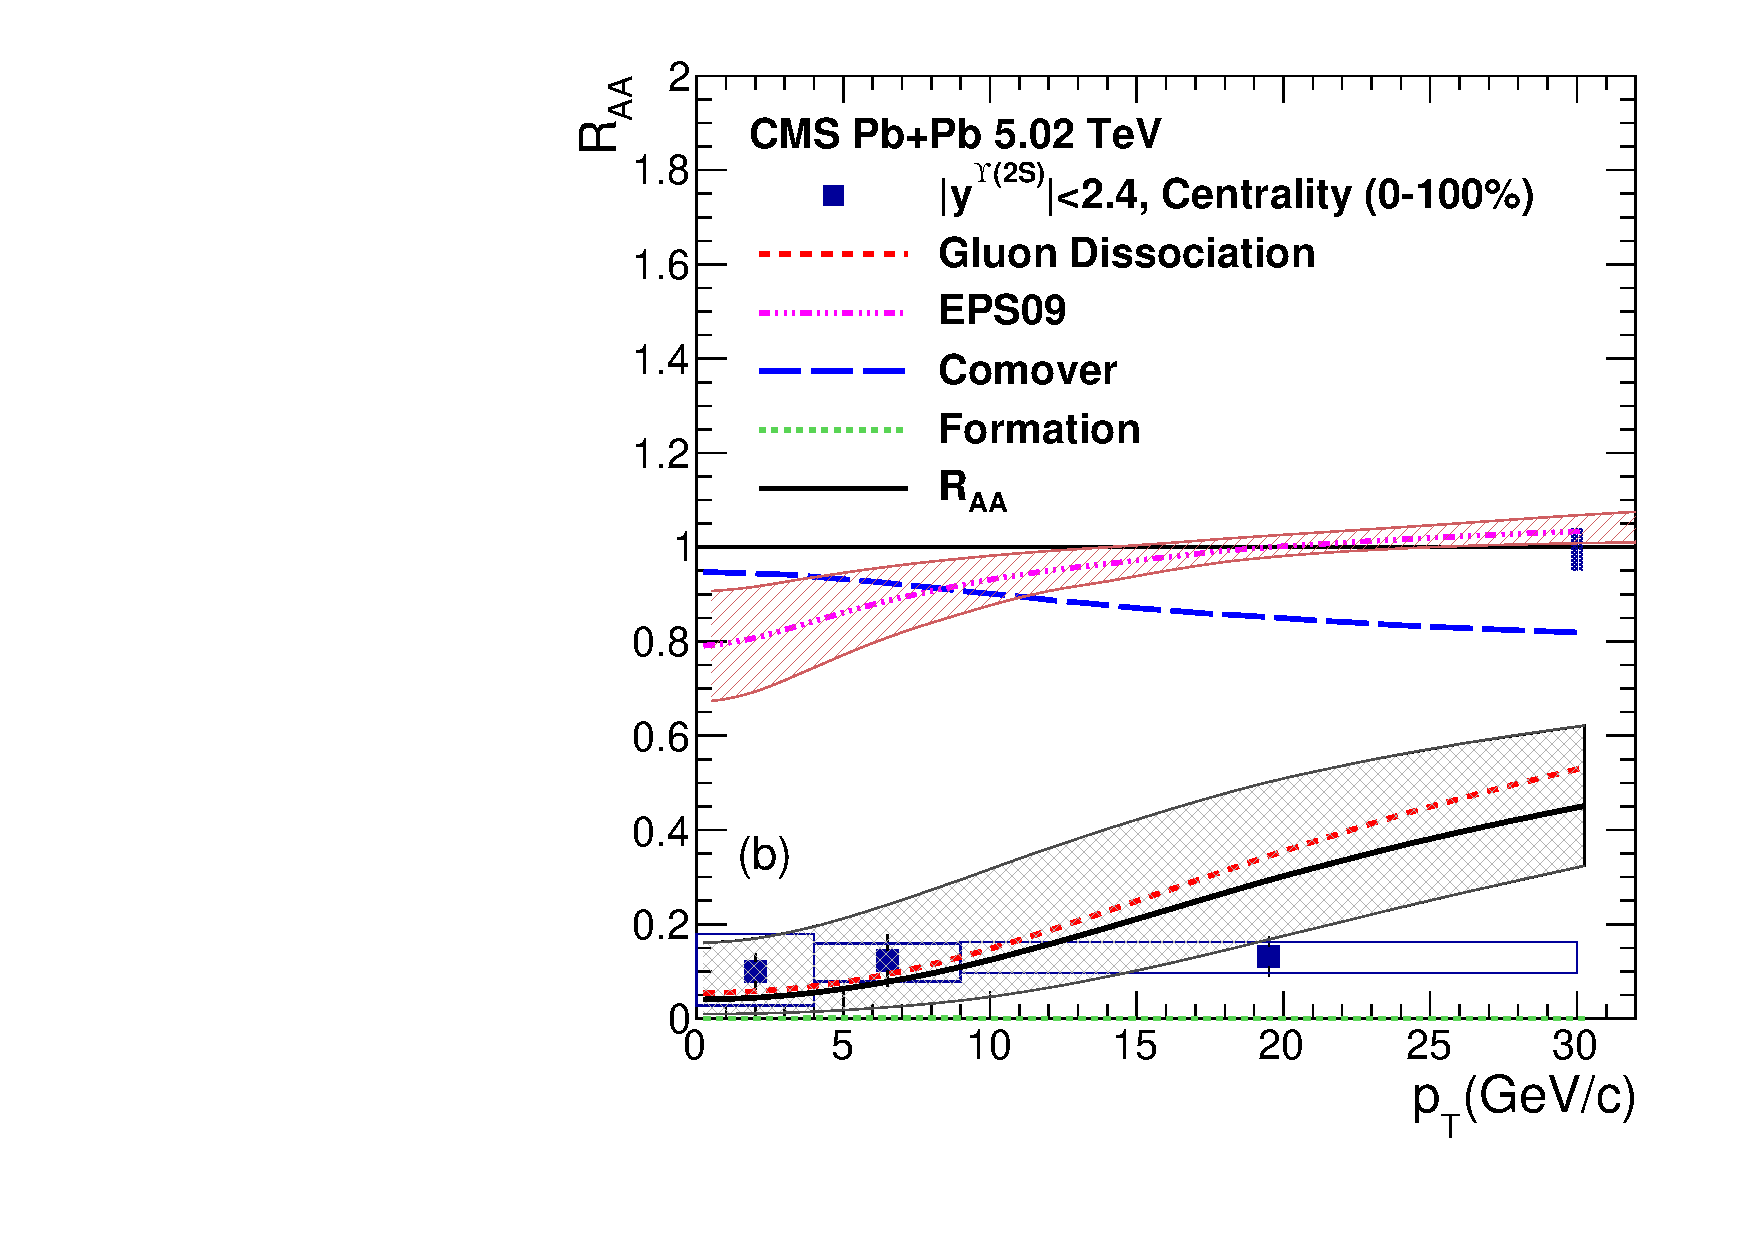
\includegraphics[width=0.49\textwidth]{Figures/Quarkonia_502TeV/Fig7b_Y2S_CMS_RAAPt_Shade.pdf}
\caption{(Color online) The $\Upsilon$(1S) azimuthal anisotropy (v$_{2}$) (a) as a function of collision centrality and 
  (b) as a function of transverse momentum $p_{T}$~\cite{CMS:2020efs}.
}
\label{fig:Upsilon1SV2CMS}
\end{figure}







\paragraph{Measurement by CMS and ATLAS}

\subsubsection{$\Upsilon$(nS) R$_{AA}$ at the RHIC}

\paragraph{Measurement by STAR and PHENIX}
